%
% 6.006 problem set 2 solutions template
%
\documentclass[12pt,twoside]{article}

\newcommand{\name}{}

\usepackage{amssymb}
\usepackage{amsmath}
\usepackage{graphicx}
\usepackage{latexsym}
\usepackage{times,url}
\usepackage{cprotect}
\usepackage{listings}
\usepackage{graphicx}
\usepackage[table]{xcolor}
\usepackage[letterpaper]{geometry}
\usepackage{tikz-qtree}
\usepackage{enumerate}

\newcommand{\profs}{Instructors: Erik Demaine, Jason Ku, and Justin Solomon}
\newcommand{\subj}{6.006}
\newcommand{\ttt}[1]{{\tt\small #1}}

\definecolor{dkgreen}{rgb}{0,0.6,0}
\definecolor{dkblue}{rgb}{.2,.2,1}
\definecolor{gray}{rgb}{0.5,0.5,0.5}
\definecolor{mauve}{rgb}{0.58,0,0.82}

\lstset{
  language=Python,
  aboveskip=1pc,
  belowskip=1pc,
  basicstyle={\footnotesize\ttfamily},
  numbers=left,
  showstringspaces=false,
  numberstyle={\tiny\color{gray}\ttfamily},
  keywordstyle={\color{dkblue}\ttfamily},
  commentstyle={\color{dkgreen}\ttfamily},
  stringstyle={\color{mauve}\ttfamily},
}

% \lstset{
%   language=Python,
%   aboveskip=1pc,
%   belowskip=1pc,
%   basicstyle={\bf\color{white}\ttfamily},
%   numbers=left,
%   showstringspaces=false,
%   numberstyle={\bf\small\color{lightgray}\ttfamily},
%   keywordstyle={\bf\color{cyan}\ttfamily},
%   commentstyle={\bf\color{green}\ttfamily},
%   stringstyle={\bf\color{mauve}\ttfamily},
% }

\tikzset{
  % every node/.style={minimum width=2em,draw,circle},
  % level 1/.style={sibling distance=2cm},
  level distance=1cm,
  edge from parent/.style=
  {draw,edge from parent path={(\tikzparentnode) -- (\tikzchildnode)}},
}
\usetikzlibrary{shapes}

\newif\ifHideSolutions
\newcommand{\solution}[1]{\color{dkgreen}\textbf{Solution: }#1\color{black}}
\newcommand{\commonmistakes}[1]{{\color{dkblue}\textbf{Common Mistakes: }#1}}
\newcommand{\rubric}[1]{\color{dkgreen}{\bf Rubric:} #1\color{black}}

% \HideSolutionsfalse
% \ifHideSolutions
%   \renewcommand{\solution}[1]{}
%   \renewcommand{\rubric}[1]{}
% \fi

\newlength{\toppush}
\setlength{\toppush}{2\headheight}
\addtolength{\toppush}{\headsep}

\newcommand{\htitle}[2]{\noindent\vspace*{-\toppush}\newline\parbox{\textwidth}
{\textit{Introduction to Algorithms: 6.006}\hfill\name\newline
Massachusetts Institute of Technology \hfill #2\newline
\profs\hfill #1 \\[-3.5ex]\newline
\mbox{}\hrulefill\mbox{}}\vspace*{1ex}\mbox{}\newline
\begin{center}{\Large\bf #1}\end{center}}

\newcommand{\handout}[2]{\thispagestyle{empty}
 \markboth{#1}{#1}
 \pagestyle{myheadings}\htitle{#1}{#2}}

\newcommand{\lecture}[3]{\thispagestyle{empty}
 \markboth{Lecture #1: #2}{Lecture #1: #2}
 \pagestyle{myheadings}\htitle{Lecture #1: #2}{#3}}

\newcommand{\htitlewithouttitle}[2]{\noindent\vspace*{-\toppush}\newline\parbox{6.5in}
{\textit{Introduction to Algorithms}\hfill#2\newline
Massachusetts Institute of Technology \hfill 6.006\newline
\profs\hfill Handout #1\vspace*{-.5ex}\newline
\mbox{}\hrulefill\mbox{}}\vspace*{1ex}\mbox{}\newline}

\newcommand{\handoutwithouttitle}[2]{\thispagestyle{empty}
 \markboth{Handout \protect\ref{#1}}{Handout \protect\ref{#1}}
 \pagestyle{myheadings}\htitlewithouttitle{\protect\ref{#1}}{#2}}

\newcommand{\exam}[2]{% parameters: exam name, date
 \thispagestyle{empty}
 \markboth{\hspace{1cm}\subj\ #1\hspace{1in}Name\hrulefill\ \ }%
          {\subj\ #1\hspace{1in}Name\hrulefill\ \ }
 \pagestyle{myheadings}\examtitle{#1}{#2}
 \renewcommand{\theproblem}{Problem \arabic{problemnum}}
}
\newcommand{\examsolutions}[3]{% parameters: handout, exam name, date
 \thispagestyle{empty}
 \markboth{Handout \protect\ref{#1}: #2}{Handout \protect\ref{#1}: #2}
% \pagestyle{myheadings}\htitle{\protect\ref{#1}}{#2}{#3}
 \pagestyle{myheadings}\examsolutionstitle{\protect\ref{#1}} {#2}{#3}
 \renewcommand{\theproblem}{Problem \arabic{problemnum}}
}
\newcommand{\examsolutionstitle}[3]{\noindent\vspace*{-\toppush}\newline\parbox{6.5in}
{\textit{Introduction to Algorithms}\hfill#3\newline
Massachusetts Institute of Technology \hfill 6.006\newline
%Singapore-MIT Alliance \hfill SMA5503\newline
\profs\hfill Handout #1\vspace*{-.5ex}\newline
\mbox{}\hrulefill\mbox{}}\vspace*{1ex}\mbox{}\newline
\begin{center}{\Large\bf #2}\end{center}}

\newcommand{\takehomeexam}[2]{% parameters: exam name, date
 \thispagestyle{empty}
 \markboth{\subj\ #1\hfill}{\subj\ #1\hfill}
 \pagestyle{myheadings}\examtitle{#1}{#2}
 \renewcommand{\theproblem}{Problem \arabic{problemnum}}
}

\makeatletter
\newcommand{\exambooklet}[2]{% parameters: exam name, date
 \thispagestyle{empty}
 \markboth{\subj\ #1}{\subj\ #1}
 \pagestyle{myheadings}\examtitle{#1}{#2}
 \renewcommand{\theproblem}{Problem \arabic{problemnum}}
 \renewcommand{\problem}{\newpage
 \item \let\@currentlabel=\theproblem
 \markboth{\subj\ #1, \theproblem}{\subj\ #1, \theproblem}}
}
\makeatother


\newcommand{\examtitle}[2]{\noindent\vspace*{-\toppush}\newline\parbox{6.5in}
{\textit{Introduction to Algorithms}\hfill#2\newline
Massachusetts Institute of Technology \hfill 6.006 Spring 2020\newline
%Singapore-MIT Alliance \hfill SMA5503\newline
\profs\hfill #1\vspace*{-.5ex}\newline
\mbox{}\hrulefill\mbox{}}\vspace*{1ex}\mbox{}\newline
\begin{center}{\Large\bf #1}\end{center}}

\newcommand{\grader}[1]{\hspace{1cm}\textsf{\textbf{#1}}\hspace{1cm}}

\newcommand{\points}[1]{[#1 points]\ }
\newcommand{\parts}[1]
{
  \ifnum#1=1
  (1 part)
  \else
  (#1 parts)
  \fi
  \ 
}

\newcommand{\bparts}{\begin{problemparts}}
\newcommand{\eparts}{\end{problemparts}}
\newcommand{\ppart}{\problempart}

%\newcommand{\lg} {lg\ }

\setlength{\oddsidemargin}{0pt}
\setlength{\evensidemargin}{0pt}
\setlength{\textwidth}{6.5in}
\setlength{\topmargin}{0in}
\setlength{\textheight}{8.5in}


\newcommand{\Spawn}{{\bf spawn} }
\newcommand{\Sync}{{\bf sync}}

\renewcommand{\cases}[1]{\left\{ \begin{array}{ll}#1\end{array}\right.}
\newcommand{\cif}[1]{\mbox{if $#1$}}
\newcommand{\cwhen}[1]{\mbox{when $#1$}}

\newcounter{problemnum}
\newcommand{\theproblem}{Problem \theproblemsetnum-\arabic{problemnum}}
\newenvironment{problems}{
        \begin{list}{{\bf \theproblem. \hspace*{0.5em}}}
        {\setlength{\leftmargin}{0em}
         \setlength{\rightmargin}{0em}
         \setlength{\labelwidth}{0em}
         \setlength{\labelsep}{0em}
         \usecounter{problemnum}}}{\end{list}}
\makeatletter
\newcommand{\problem}[1][{}]{\item \let\@currentlabel=\theproblem \textbf{#1}}
\makeatother

\newcounter{problempartnum}[problemnum]
\newenvironment{problemparts}{
        \begin{list}{{\bf (\alph{problempartnum})}}
        {\setlength{\leftmargin}{2.5em}
         \setlength{\rightmargin}{2.5em}
         \setlength{\labelsep}{0.5em}}}{\end{list}}
\newcommand{\problempart}{\addtocounter{problempartnum}{1}\item}

\newenvironment{truefalseproblemparts}{
        \begin{list}{{\bf (\alph{problempartnum})\ \ \ T\ \ F\hfil}}
        {\setlength{\leftmargin}{4.5em}
         \setlength{\rightmargin}{2.5em}
         \setlength{\labelsep}{0.5em}
         \setlength{\labelwidth}{4.5em}}}{\end{list}}

\newcounter{exercisenum}
\newcommand{\theexercise}{Exercise \theproblemsetnum-\arabic{exercisenum}}
\newenvironment{exercises}{
        \begin{list}{{\bf \theexercise. \hspace*{0.5em}}}
        {\setlength{\leftmargin}{0em}
         \setlength{\rightmargin}{0em}
         \setlength{\labelwidth}{0em}
         \setlength{\labelsep}{0em}
        \usecounter{exercisenum}}}{\end{list}}
\makeatletter
\newcommand{\exercise}{\item \let\@currentlabel=\theexercise}
\makeatother

\newcounter{exercisepartnum}[exercisenum]
%\newcommand{\problem}[1]{\medskip\mbox{}\newline\noindent{\bf Problem #1.}\hspace*{1em}}
%\newcommand{\exercise}[1]{\medskip\mbox{}\newline\noindent{\bf Exercise #1.}\hspace*{1em}}

\newenvironment{exerciseparts}{
        \begin{list}{{\bf (\alph{exercisepartnum})}}
        {\setlength{\leftmargin}{2.5em}
         \setlength{\rightmargin}{2.5em}
         \setlength{\labelsep}{0.5em}}}{\end{list}}
\newcommand{\exercisepart}{\addtocounter{exercisepartnum}{1}\item}


% Macros to make captions print with small type and 'Figure xx' in bold.
\makeatletter
\def\fnum@figure{{\bf Figure \thefigure}}
\def\fnum@table{{\bf Table \thetable}}
\let\@mycaption\caption
%\long\def\@mycaption#1[#2]#3{\addcontentsline{\csname
%  ext@#1\endcsname}{#1}{\protect\numberline{\csname 
%  the#1\endcsname}{\ignorespaces #2}}\par
%  \begingroup
%    \@parboxrestore
%    \small
%    \@makecaption{\csname fnum@#1\endcsname}{\ignorespaces #3}\par
%  \endgroup}
%\def\mycaption{\refstepcounter\@captype \@dblarg{\@mycaption\@captype}}
%\makeatother
\let\mycaption\caption
%\newcommand{\figcaption}[1]{\mycaption[]{#1}}

\newcounter{totalcaptions}
\newcounter{totalart}

\newcommand{\figcaption}[1]{\addtocounter{totalcaptions}{1}\caption[]{#1}}

% \psfigures determines what to do for figures:
%       0 means just leave vertical space
%       1 means put a vertical rule and the figure name
%       2 means insert the PostScript version of the figure
%       3 means put the figure name flush left or right
\newcommand{\psfigures}{0}
\newcommand{\spacefigures}{\renewcommand{\psfigures}{0}}
\newcommand{\rulefigures}{\renewcommand{\psfigures}{1}}
\newcommand{\macfigures}{\renewcommand{\psfigures}{2}}
\newcommand{\namefigures}{\renewcommand{\psfigures}{3}}

\newcommand{\figpart}[1]{{\bf (#1)}\nolinebreak[2]\relax}
\newcommand{\figparts}[2]{{\bf (#1)--(#2)}\nolinebreak[2]\relax}


\macfigures     % STATE

% When calling \figspace, make sure to leave a blank line afterward!!
% \widefigspace is for figures that are more than 28pc wide.
\newlength{\halffigspace} \newlength{\wholefigspace}
\newlength{\figruleheight} \newlength{\figgap}
\newcommand{\setfiglengths}{\ifnum\psfigures=1\setlength{\figruleheight}{\hruleheight}\setlength{\figgap}{1em}\else\setlength{\figruleheight}{0pt}\setlength{\figgap}{0em}\fi}
\newcommand{\figspace}[2]{\ifnum\psfigures=0\leavefigspace{#1}\else%
\setfiglengths%
\setlength{\wholefigspace}{#1}\setlength{\halffigspace}{.5\wholefigspace}%
\rule[-\halffigspace]{\figruleheight}{\wholefigspace}\hspace{\figgap}#2\fi}
\newlength{\widefigspacewidth}
% Make \widefigspace put the figure flush right on the text page.
\newcommand{\widefigspace}[2]{
\ifnum\psfigures=0\leavefigspace{#1}\else%
\setfiglengths%
\setlength{\widefigspacewidth}{28pc}%
\addtolength{\widefigspacewidth}{-\figruleheight}%
\setlength{\wholefigspace}{#1}\setlength{\halffigspace}{.5\wholefigspace}%
\makebox[\widefigspacewidth][r]{#2\hspace{\figgap}}\rule[-\halffigspace]{\figruleheight}{\wholefigspace}\fi}
\newcommand{\leavefigspace}[1]{\setlength{\wholefigspace}{#1}\setlength{\halffigspace}{.5\wholefigspace}\rule[-\halffigspace]{0em}{\wholefigspace}}

% Commands for including figures with macpsfig.
% To use these commands, documentstyle ``macpsfig'' must be specified.
\newlength{\macfigfill}
\makeatother
\newlength{\bbx}
\newlength{\bby}
\newcommand{\macfigure}[5]{\addtocounter{totalart}{1}
\ifnum\psfigures=2%
\setlength{\bbx}{#2}\addtolength{\bbx}{#4}%
\setlength{\bby}{#3}\addtolength{\bby}{#5}%
\begin{flushleft}
\ifdim#4>28pc\setlength{\macfigfill}{#4}\addtolength{\macfigfill}{-28pc}\hspace*{-\macfigfill}\fi%
\mbox{\psfig{figure=./#1.ps,%
bbllx=#2,bblly=#3,bburx=\bbx,bbury=\bby}}
\end{flushleft}%
\else\ifdim#4>28pc\widefigspace{#5}{#1}\else\figspace{#5}{#1}\fi\fi}
\makeatletter

\newlength{\savearraycolsep}
\newcommand{\narrowarray}[1]{\setlength{\savearraycolsep}{\arraycolsep}\setlength{\arraycolsep}{#1\arraycolsep}}
\newcommand{\normalarray}{\setlength{\arraycolsep}{\savearraycolsep}}

\newcommand{\hint}{{\bf Hint:\ }}

% Macros from /th/u/clr/mac.tex

\newcommand{\set}[1]{\left\{ #1 \right\}}
\newcommand{\abs}[1]{\left| #1\right|}
\newcommand{\card}[1]{\left| #1\right|}
\newcommand{\floor}[1]{\left\lfloor #1 \right\rfloor}
\newcommand{\ceil}[1]{\left\lceil #1 \right\rceil}
\newcommand{\ang}[1]{\ifmmode{\left\langle #1 \right\rangle}
   \else{$\left\langle${#1}$\right\rangle$}\fi}
        % the \if allows use outside mathmode,
        % but will swallow following space there!
\newcommand{\paren}[1]{\left( #1 \right)}
\newcommand{\bracket}[1]{\left[ #1 \right]}
\newcommand{\prob}[1]{\Pr\left\{ #1 \right\}}
\newcommand{\Var}{\mathop{\rm Var}\nolimits}
\newcommand{\expect}[1]{{\rm E}\left[ #1 \right]}
\newcommand{\expectsq}[1]{{\rm E}^2\left[ #1 \right]}
\newcommand{\variance}[1]{{\rm Var}\left[ #1 \right]}
\renewcommand{\choose}[2]{{{#1}\atopwithdelims(){#2}}}
\def\pmod#1{\allowbreak\mkern12mu({\rm mod}\,\,#1)}
\newcommand{\matx}[2]{\left(\begin{array}{*{#1}{c}}#2\end{array}\right)}
\newcommand{\Adj}{\mathop{\rm Adj}\nolimits}

\newtheorem{theorem}{Theorem}
\newtheorem{lemma}[theorem]{Lemma}
\newtheorem{corollary}[theorem]{Corollary}
\newtheorem{xample}{Example}
\newtheorem{definition}{Definition}
\newenvironment{example}{\begin{xample}\rm}{\end{xample}}
\newcommand{\proof}{\noindent{\em Proof.}\hspace{1em}}
\def\squarebox#1{\hbox to #1{\hfill\vbox to #1{\vfill}}}
\newcommand{\qedbox}{\vbox{\hrule\hbox{\vrule\squarebox{.667em}\vrule}\hrule}}
\newcommand{\qed}{\nopagebreak\mbox{}\hfill\qedbox\smallskip}
\newcommand{\eqnref}[1]{(\protect\ref{#1})}

%%\newcommand{\twodots}{\mathinner{\ldotp\ldotp}}
\newcommand{\transpose}{^{\mbox{\scriptsize \sf T}}}
\newcommand{\amortized}[1]{\widehat{#1}}

\newcommand{\punt}[1]{}

%%% command for putting definitions into boldface
% New style for defined terms, as of 2/23/88, redefined by THC.
\newcommand{\defn}[1]{{\boldmath\textit{\textbf{#1}}}}
\newcommand{\defi}[1]{{\textit{\textbf{#1\/}}}}

\newcommand{\red}{\leq_{\rm P}}
\newcommand{\lang}[1]{%
\ifmmode\mathord{\mathcode`-="702D\rm#1\mathcode`\-="2200}\else{\rm#1}\fi}

%\newcommand{\ckt}[1]{\ifmmode\mathord{\mathcode`-="702D\sc #1\mathcode`\-="2200}\else$\mathord{\mathcode`-="702D\sc #1\mathcode`\-="2200}$\fi}
\newcommand{\ckt}[1]{\ifmmode \sc #1\else$\sc #1$\fi}

%% Margin notes - use \notesfalse to turn off notes.
\setlength{\marginparwidth}{0.6in}
\reversemarginpar
\newif\ifnotes
\notestrue
\newcommand{\longnote}[1]{
  \ifnotes
    {\medskip\noindent Note: \marginpar[\hfill$\Longrightarrow$]
      {$\Longleftarrow$}{#1}\medskip}
  \fi}
\newcommand{\note}[1]{
  \ifnotes
    {\marginpar{\tiny \raggedright{#1}}}
  \fi}


\newcommand{\reals}{\mathbbm{R}}
\newcommand{\integers}{\mathbbm{Z}}
\newcommand{\naturals}{\mathbbm{N}}
\newcommand{\rationals}{\mathbbm{Q}}
\newcommand{\complex}{\mathbbm{C}}

\newcommand{\oldreals}{{\bf R}}
\newcommand{\oldintegers}{{\bf Z}}
\newcommand{\oldnaturals}{{\bf N}}
\newcommand{\oldrationals}{{\bf Q}}
\newcommand{\oldcomplex}{{\bf C}}

\newcommand{\w}{\omega}                 %% for fft chapter

\newenvironment{closeitemize}{\begin{list}
{$\bullet$}
{\setlength{\itemsep}{-0.2\baselineskip}
\setlength{\topsep}{0.2\baselineskip}
\setlength{\parskip}{0pt}}}
{\end{list}}

% These are necessary within a {problems} environment in order to restore
% the default separation between bullets and items.
\newenvironment{normalitemize}{\setlength{\labelsep}{0.5em}\begin{itemize}}
                              {\end{itemize}}
\newenvironment{normalenumerate}{\setlength{\labelsep}{0.5em}\begin{enumerate}}
                                {\end{enumerate}}

%\def\eqref#1{Equation~(\ref{eq:#1})}
%\newcommand{\eqref}[1]{Equation (\ref{eq:#1})}
\newcommand{\eqreftwo}[2]{Equations (\ref{eq:#1}) and~(\ref{eq:#2})}
\newcommand{\ineqref}[1]{Inequality~(\ref{ineq:#1})}
\newcommand{\ineqreftwo}[2]{Inequalities (\ref{ineq:#1}) and~(\ref{ineq:#2})}

\newcommand{\figref}[1]{Figure~\ref{fig:#1}}
\newcommand{\figreftwo}[2]{Figures \ref{fig:#1} and~\ref{fig:#2}}

\newcommand{\liref}[1]{line~\ref{li:#1}}
\newcommand{\Liref}[1]{Line~\ref{li:#1}}
\newcommand{\lirefs}[2]{lines \ref{li:#1}--\ref{li:#2}}
\newcommand{\Lirefs}[2]{Lines \ref{li:#1}--\ref{li:#2}}
\newcommand{\lireftwo}[2]{lines \ref{li:#1} and~\ref{li:#2}}
\newcommand{\lirefthree}[3]{lines \ref{li:#1}, \ref{li:#2}, and~\ref{li:#3}}

\newcommand{\lemlabel}[1]{\label{lem:#1}}
\newcommand{\lemref}[1]{Lemma~\ref{lem:#1}} 

\newcommand{\exref}[1]{Exercise~\ref{ex:#1}}

\newcommand{\handref}[1]{Handout~\ref{#1}}

\newcommand{\defref}[1]{Definition~\ref{def:#1}}

% (1997.8.16: Victor Luchangco)
% Modified \hlabel to only get date and to use handouts counter for number.
%   New \handout and \handoutwithouttitle commands in newmac.tex use this.
%   The date is referenced by <label>-date.
%   (Retained old definition as \hlabelold.)
%   Defined \hforcelabel to use an argument instead of the handouts counter.

\newcounter{handouts}
\setcounter{handouts}{0}

\newcommand{\hlabel}[2]{%
\stepcounter{handouts}
{\edef\next{\write\@auxout{\string\newlabel{#1}{{\arabic{handouts}}{0}}}}\next}
\write\@auxout{\string\newlabel{#1-date}{{#2}{0}}}
}

\newcommand{\hforcelabel}[3]{%          Does not step handouts counter.
\write\@auxout{\string\newlabel{#1}{{#2}{0}}}
\write\@auxout{\string\newlabel{#1-date}{{#3}{0}}}}


% less ugly underscore
% --juang, 2008 oct 05
\renewcommand{\_}{\vrule height 0 pt depth 0.4 pt width 0.5 em \,}

% multiline framed box (will always extend to the far right edge; for a short single line, use \fbox directly)
% --zabel, fall 2018
\newcommand\framepar[1]{\fbox{\begin{minipage}{\linewidth}#1\end{minipage}}}


\newcommand{\theproblemsetnum}{2}

\title{6.006 Problem Set 2}

\begin{document}

\handout{Problem Set \theproblemsetnum}

\setlength{\parindent}{0pt}
\medskip\hrulefill\medskip

{\bf Name:} Your Name

\medskip

{\bf Collaborators:} Name1, Name2

\medskip\hrulefill

%%%%%%%%%%%%%%%%%%%%%%%%%%%%%%%%%%%%%%%%%%%%%%%%%%%%%
% See below for common and useful latex constructs. %
%%%%%%%%%%%%%%%%%%%%%%%%%%%%%%%%%%%%%%%%%%%%%%%%%%%%%

% Some useful commands:
%$f(x) = \Theta(x)$
%$T(x, y) \leq \log(x) + 2^y + \binom{2n}{n}$
% {\tt code\_function}


% You can create unnumbered lists as follows:
%\begin{itemize}
%    \item First item in a list
%        \begin{itemize}
%            \item First item in a list
%                \begin{itemize}
%                    \item First item in a list
%                    \item Second item in a list
%                \end{itemize}
%            \item Second item in a list
%        \end{itemize}
%    \item Second item in a list
%\end{itemize}

% You can create numbered lists as follows:
%\begin{enumerate}
%    \item First item in a list
%    \item Second item in a list
%    \item Third item in a list
%\end{enumerate}

% You can write aligned equations as follows:
%\begin{align}
%    \begin{split}
%        (x+y)^3 &= (x+y)^2(x+y) \\
%                &= (x^2+2xy+y^2)(x+y) \\
%                &= (x^3+2x^2y+xy^2) + (x^2y+2xy^2+y^3) \\
%                &= x^3+3x^2y+3xy^2+y^3
%    \end{split}
%\end{align}

% You can create grids/matrices as follows:
%\begin{align}
%    A =
%    \begin{bmatrix}
%        A_{11} & A_{21} \\
%        A_{21} & A_{22}
%    \end{bmatrix}
%\end{align}

% You can include images and PDFs as follows:
% 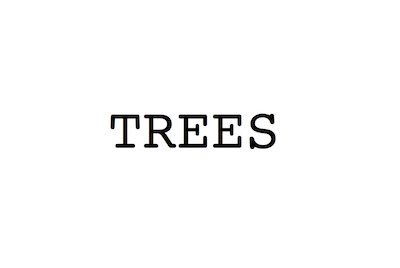
\includegraphics[width=0.5\textwidth]{img.jpg}

\begin{problems}

\problem  % Problem 1

\begin{problemparts}
\problempart % Problem 1a
$T(n) = 4T(n/2) + O(n)$. \textbf{Recursion tree:} level $i$ has $4^i$ nodes, each on a
subproblem of size $n/2^i$, so each costs at most $cn/2^i$.

\begin{center}
\begin{tabular}{c|c|c|c}
level & nodes & work per node & work in level \\ \hline
$0$ & $1$ & $cn$ & $cn$ \\
$1$ & $4$ & $cn/2$ & $2cn$ \\
$i$ & $4^i$ & $cn/2^i$ & $2^i cn$ \\
$\lg n$ (leaves) & $4^{\lg n} = n^2$ & $\Theta(1)$ & $\Theta(n^2)$
\end{tabular}
\end{center}

The level costs grow geometrically, so the total is at most
$cn\sum_{i=0}^{\lg n}2^i < 2cn\cdot n = O(n^2)$. The $n^2$ leaves alone cost
$\Omega(n^2)$. So $T(n) = \Theta(n^2)$.

\textbf{Master Theorem:} $a=4$, $b=2$, so $n^{\log_b a} = n^2$. Since $f(n)=O(n)=O(n^{2-\varepsilon})$
with $\varepsilon = 1$, case 1 gives $T(n)=\Theta(n^2)$.

\problempart % Problem 1b
$T(n) = 3T(n/\sqrt2) + O(n^4)$. \textbf{Recursion tree:} level $i$ has $3^i$ nodes of size
$n/2^{i/2}$, each costing at most $c\,n^4/4^i$.

\begin{center}
\begin{tabular}{c|c|c|c}
level & nodes & work per node & work in level \\ \hline
$0$ & $1$ & $cn^4$ & $cn^4$ \\
$i$ & $3^i$ & $cn^4/4^i$ & $(3/4)^i cn^4$ \\
last & $3^{2\lg n} = n^{2\lg 3}$ & $\Theta(1)$ & $\Theta(n^{2\lg 3})$
\end{tabular}
\end{center}

The level costs shrink geometrically, so the total is at most
$cn^4\sum_{i\ge 0}(3/4)^i = 4cn^4$, giving $T(n)=O(n^4)$. The leaves alone cost
$\Omega(n^{2\lg 3})$, giving $T(n)=\Omega(n^{2\lg 3})$ (note $2\lg 3\approx 3.17 < 4$).

\textbf{Master Theorem:} $a=3$, $b=\sqrt2$, so $n^{\log_b a}=n^{2\lg 3}$. For the upper bound
take $f(n)=n^4$: $f(n)=\Omega(n^{2\lg 3+\varepsilon})$ for $\varepsilon \le 4-2\lg 3$, and
$3f(n/\sqrt2) = \tfrac34 n^4 \le c f(n)$ with $c = 3/4 < 1$, so case 3 gives $O(n^4)$.
For the lower bound take $f(n)=0$: case 1 gives $\Omega(n^{2\lg 3})$.
(Since $f$ is only bounded above by $O(n^4)$, these are the tightest bounds the recurrence allows.)

\problempart % Problem 1c
$T(n) = 2T(n/2) + 5n\log n$. \textbf{Recursion tree:} level $i$ has $2^i$ nodes of size $n/2^i$,
each costing $5\frac{n}{2^i}\log\frac{n}{2^i}$.

\begin{center}
\begin{tabular}{c|c|c|c}
level & nodes & work per node & work in level \\ \hline
$0$ & $1$ & $5n\log n$ & $5n\log n$ \\
$i$ & $2^i$ & $5\frac{n}{2^i}(\log n - i)$ & $5n(\log n - i)$ \\
$\lg n$ (leaves) & $n$ & $\Theta(1)$ & $\Theta(n)$
\end{tabular}
\end{center}

Substituting $j=\log n - i$ and summing over all levels:
$\sum_{j=0}^{\log n} 5nj = 5n\,\frac{\log n(\log n+1)}{2} = \Theta(n\log^2 n)$.

\textbf{Master Theorem:} $a=b=2$, so $n^{\log_b a}=n$, and $f(n)=5n\log n=\Theta(n\log^1 n)$.
This is case 2 with $k=1$, so $T(n)=\Theta(n\log^2 n)$.

\problempart % Problem 1d
$T(n) = T(n-2)+\Theta(n)$, by substitution. Say the $\Theta(n)$ term lies between $d_1 n$ and
$d_2 n$. Guess $T(n)=\Theta(n^2)$.

\emph{Upper bound:} assume $T(m)\le cm^2$ for $m<n$. Then
$T(n)\le c(n-2)^2 + d_2 n = cn^2 - 4cn + 4c + d_2 n \le cn^2$
whenever $4cn - 4c \ge d_2 n$, which holds for $n\ge 2$ if $c \ge d_2/2$.

\emph{Lower bound:} assume $T(m)\ge cm^2$ for $m<n$. Then
$T(n)\ge c(n-2)^2 + d_1 n = cn^2 - 4cn + 4c + d_1 n \ge cn^2$
whenever $d_1 n \ge 4cn$, which holds if $c \le d_1/4$.

The base case $T(1)=\Theta(1)$ is fine for a small enough $c$ (lower) and large enough $c$ (upper).
Hence $T(n)=\Theta(n^2)$.
\end{problemparts}

\newpage
\problem  % Problem 2

\begin{problemparts}
\problempart % Problem 2a
\textbf{Selection sort.} The sort must be in-place, which rules out merge sort. Of the other two,
what matters is the number of \texttt{set\_at} calls, since each costs $\Theta(n\log n)$ while
\texttt{get\_at} is $\Theta(1)$. Insertion sort may do $\Theta(n^2)$ \texttt{set\_at} calls (every
shift is a write), for $O(n^2\cdot n\log n)=O(n^3\log n)$. Selection sort does $O(n^2)$ reads but
only $O(n)$ writes (one swap per round), for $O(n^2 + n\cdot n\log n)=O(n^2\log n)$.

\problempart % Problem 2b
\textbf{Merge sort.} Reads/writes of pointers are $O(1)$, but each comparison costs $\Theta(\log n)$,
so what matters is the number of comparisons. Selection and insertion sort need $\Theta(n^2)$
comparisons in the worst case, so $\Theta(n^2\log n)$ total. Merge sort needs only $O(n\log n)$
comparisons, so $O(n\log^2 n)$ total, which is better.

\problempart % Problem 2c
\textbf{Insertion sort.} Selection sort always takes $\Theta(n^2)$ and merge sort always takes
$\Theta(n\log n)$, whatever the input. Insertion sort's inner loop stops as soon as an item is in
place, so its running time is $O(n + I)$ where $I$ is the number of inversions (each inner-loop
swap removes exactly one inversion). One swap of adjacent items changes the number of inversions
by at most one, so after $\log\log n$ such swaps $I\le \log\log n$. Then insertion sort runs in
$O(n+\log\log n)=O(n)$ time, which beats $\Theta(n\log n)$.
\end{problemparts}

\newpage
\problem  % Problem 3

\textbf{Idea:} search from both ends at once with exponentially growing steps (like exponential
search), stop as soon as Datum is bracketed, then binary search the bracket.

\textbf{Algorithm.} For $i=0,1,2,\dots$:
\begin{enumerate}
\item Teleport to kilometer $2^i$ (counted from the north end) and use the tracker. If Datum is
here, done. If Datum is \emph{north} of here, he lies in $(2^{i-1},2^i)$: stop and binary search
that range.
\item Otherwise teleport to kilometer $n-2^i$. If Datum is here, done. If Datum is \emph{south}
of here, he lies in $(n-2^i,\,n-2^{i-1})$: stop and binary search that range.
\item Otherwise continue with $i+1$.
\end{enumerate}
(For $i=0$ the ``previous'' probe is the end of the island itself.)

\textbf{Correctness.} Suppose Datum is at distance $k$ from the nearest end, and say it is the north
end ($k\le n/2$; the south case is symmetric). For every $i$ with $2^i<k$, the north probe says
``south'' and the south probe (at $n-2^i > k$) says ``north'', so nothing triggers. At the first
$i$ with $2^i\ge k$ the north probe finds him or reports ``north'', and since he was south of
$2^{i-1}$ he is bracketed in $(2^{i-1},2^i)$. The south probes cannot stop the search earlier,
because Datum is never south of $n-2^{i}$ while $2^i<n-k$, and $2^i < 2k \le n$ at that point.
Binary search on a bracket that contains Datum then returns his exact kilometer.

\textbf{Running time.} The first $i$ with $2^i\ge k$ satisfies $i=\lceil\lg k\rceil$, so we make at
most $2(i+1)=O(\log k)$ probes in the doubling phase. The bracket has fewer than $2^{i-1}<k$
kilometers, so binary search uses $O(\log k)$ more probes. Total $O(\log k)$.

\newpage
\problem  % Problem 4

\textbf{Data structure.} Keep two things:
\begin{itemize}
\item a doubly linked list $L$ of all \emph{undeleted} messages, in the order they were sent
(oldest at the head, newest at the tail);
\item an array $S$ of the $n$ viewer IDs, sorted by ID. Each entry $S[j]$ stores the viewer's ID
and a pointer to that viewer's own singly linked list $L_v$, whose nodes point to the nodes of $L$
holding $v$'s messages. A \texttt{None} pointer in place of $L_v$ means $v$ is banned.
\end{itemize}

\textbf{build($V$).} Put the $n$ IDs into $S$ with an empty $L_v$ each ($O(n)$), set $L$ to empty
($O(1)$), and sort $S$ by ID with merge sort ($O(n\log n)$). Worst-case $O(n\log n)$.

\textbf{send($v,m$).} Binary search $S$ for $v$ in $O(\log n)$. If $L_v$ is \texttt{None}, the
viewer is banned and nothing happens. Otherwise append a new node $x$ holding $m$ at the tail of
$L$ ($O(1)$) and insert a pointer to $x$ at the front of $L_v$ ($O(1)$). Worst-case $O(\log n)$.

\textbf{recent($k$).} Start at the tail of $L$ and walk backward through $\min(k,|L|)$ nodes,
returning their messages. Since $L$ contains exactly the undeleted messages in order, these are
the $k$ most recent ones. Worst-case $O(k)$.

\textbf{ban($v$).} Binary search $S$ for $v$ in $O(\log n)$. For each of the $n_v$ pointers in
$L_v$, unlink the node it points to from $L$; this is $O(1)$ each because $L$ is doubly linked,
so no search is needed. Finally set $v$'s pointer in $S$ to \texttt{None} (and drop $L_v$).
Worst-case $O(n_v+\log n)$.

All invariants hold after each operation: $L$ always holds exactly the messages of non-banned
viewers in sending order, and each $L_v$ points to exactly the nodes of $L$ sent by $v$.

\newpage
\problem  % Problem 5

\begin{problemparts}
\problempart % Problem 5a
Think of a booking schedule as a step function ``number of rooms in use at time $x$''. Booking
$(k,s,t)$ means the function goes up by $k$ at time $s$ and down by $k$ at time $t$. The step
function of $R_1\cup R_2$ is the \emph{sum} of the two step functions, so we can compute it by
merging their change points.

\textbf{Algorithm.}
\begin{enumerate}
\item Turn each schedule into a list of events $(\text{time},\text{change})$: each booking
$(k,s,t)$ gives $(s,+k)$ and $(t,-k)$. Because bookings in a schedule are disjoint and sorted,
each event list is already sorted by time.
\item Merge the two sorted event lists into one sorted list $E$, as in merge sort.
\item Sweep through $E$ keeping the current room count $c$ (initially $0$) and the time
$\mathit{start}$ of the current stretch. Take all events with the same time $T$ together and let
$\delta$ be the sum of their changes. If $\delta\neq 0$: if $c>0$, output booking
$(c,\mathit{start},T)$; then set $c\gets c+\delta$ and $\mathit{start}\gets T$.
If $\delta=0$, do nothing.
\end{enumerate}

\textbf{Correctness.} Between two consecutive times where the count changes, the number of rooms in
use is constant and equals $c$, so a booking $(c,\mathit{start},T)$ is output exactly for each
maximal stretch with $c>0$. Skipping times with $\delta=0$ means two neighbouring stretches with the
same count are never split (so adjacent bookings have different room counts), and stretches with
$c=0$ produce no booking. The result is therefore the unique satisfying schedule for
$R_1\cup R_2$, with bookings disjoint and in increasing order.

\textbf{Running time.} There are $2n$ events. Building the lists, merging, and sweeping each take
$O(n)$ time, so the total is $O(n)$.

\problempart % Problem 5b
Use divide and conquer. If $|R|=1$ with $R=\{(s,t)\}$, return $((1,s,t))$. Otherwise split $R$ into
two halves $R_1,R_2$ of sizes $\lfloor n/2\rfloor$ and $\lceil n/2\rceil$, recursively compute
their satisfying schedules $B_1,B_2$, and combine them with the merge from part (a).

\textbf{Correctness} follows by induction on $|R|$: the base case is clearly satisfying, and
part (a) turns satisfying schedules of $R_1,R_2$ into a satisfying schedule of $R_1\cup R_2$.

\textbf{Running time.} A schedule for $m$ requests has at most $2m-1$ bookings, so the merge at size
$n$ costs $O(n)$ and $T(n)=2T(n/2)+O(n)$. By Master Theorem case 2, $T(n)=\Theta(n\log n)$.

\problempart Submit your implementation to {\small\url{alg.mit.edu}}.

\begin{verbatim}
def merge_bookings(B1, B2):
    # booking -> events (time, change in rooms); output is time-sorted
    def events(B):
        ev = []
        for k, s, t in B:
            ev.append((s, k))
            ev.append((t, -k))
        return ev
    E1, E2 = events(B1), events(B2)
    # standard two-pointer merge of two sorted lists
    E, a, b = [], 0, 0
    while a < len(E1) or b < len(E2):
        if b == len(E2) or (a < len(E1) and E1[a][0] <= E2[b][0]):
            E.append(E1[a]); a += 1
        else:
            E.append(E2[b]); b += 1
    # sweep: group events at equal times; emit booking when count changes
    B, rooms, start, i = [], 0, 0, 0
    while i < len(E):
        T, delta = E[i]
        i += 1
        while i < len(E) and E[i][0] == T:
            delta += E[i][1]
            i += 1
        if delta != 0:
            if rooms > 0:
                B.append((rooms, start, T))
            rooms += delta
            start = T
    return B

def satisfying_booking(R):
    if len(R) == 1:
        s, t = R[0]
        return ((1, s, t),)
    m = len(R) // 2
    B1 = satisfying_booking(R[:m])
    B2 = satisfying_booking(R[m:])
    return tuple(merge_bookings(B1, B2))
\end{verbatim}
\end{problemparts}

\end{problems}

\end{document}
